\documentclass[iop]{emulateapj-rtx4}


%\documentclass[12pt]{article}
%\pdfpagewidth 8.5in
%\pdfpageheight 11in 
%\setlength\topmargin{0in}
%\setlength\headheight{0in}
%\setlength\headsep{0in}
%\setlength\textheight{9in}
%\setlength\textwidth{6.5in}
%\setlength\oddsidemargin{0in}
%\setlength\evensidemargin{0in}

\usepackage{graphicx}
\usepackage{amssymb}


%\usepackage{multicol}
%\usepackage{sidecap}
%\usepackage{ragged2e}

%\usepackage{caption}
%\usepackage{subcaption}

%\usepackage{subfig}
\usepackage{wrapfig}
\usepackage{setspace}
\usepackage{subfigure}
\usepackage{mathtools}


%\newcommand{\rms}[1]{\langle #1 \rangle}
%\renewcommand{\baselinestretch}{1.5}
%\renewcommand{\thefootnote}{\roman{footnote}}

\newcommand{\kms}{$\rm km\, s^{-1}$}


\graphicspath{{gt_figures//}}


\frenchspacing

\begin{document}


\title{A New Nearby Galaxy Table\textsuperscript{*}}

\author{David M. French, Bart P. Wakker}

\affil{Department of Astronomy, University of Wisconsin - Madison}


\begin{abstract}

We present an all-sky catalog of galaxies in the nearby, $cz \leq 10,000$ \kms~ redshift range. 

\end{abstract}
\keywords{IGM, CGM, galaxies}


\section{Introduction}
Galaxy catalogs at once seem somewhat outdated in the age of the internet, yet still frustratingly necessary. The ideal solution of an all-sky and all-object online database containing homogenized information has not been completely realized, even as the NASA Extragalactic Database (NED), Vizier, SIMBAD and others fulfill some of these requirements. Each of these databases offer slightly different sets of information on their objects however, and there is often no straightforward way for extracting all the parameters needed. For example, there is no way to return the diameters of all known galaxies in a particular redshift range.


Some background on currently available, up to date catalogs.

Is anything missing? What hole are we filling with this one?

At the risk of creating yet another catalog 

In an effort to study the circumgalactic medium (CGM) in the nearby universe we have constructed a catalog of galaxies with $cz \leq 10,000$ \kms. All of the data included here is publicly available through the NASA Extragalactic Database (NED) and the NASA/IPAC Infrared Science Archive (IRSA). We have endeavored in various ways to create a single, homogeneous catalog 

This catalog is not meant to be entirely robust or comprehensive - rather it's purpose is to present a common batch of parameters for nearby galaxies in a easily retrievable and machine-readable manner. We have nonetheless endeavored to provide reasonable error estimates on all derivations and for as many observed quantities as possible.


\section{Data}

\subsection{Galaxy Data Retrieval}

The goal of this study relies on knowing the locations and properties of all galaxies near detected Ly$\alpha$ absorption lines. To facilitate this, we have constructed a dataset of all $z\leq 0.033$ ($cz\leq 10,000$ \kms) galaxies with published data available through the NASA Extragalactic Database (NED). 

\begin{figure}[ht!]
        \centering
        \vspace{0pt}
        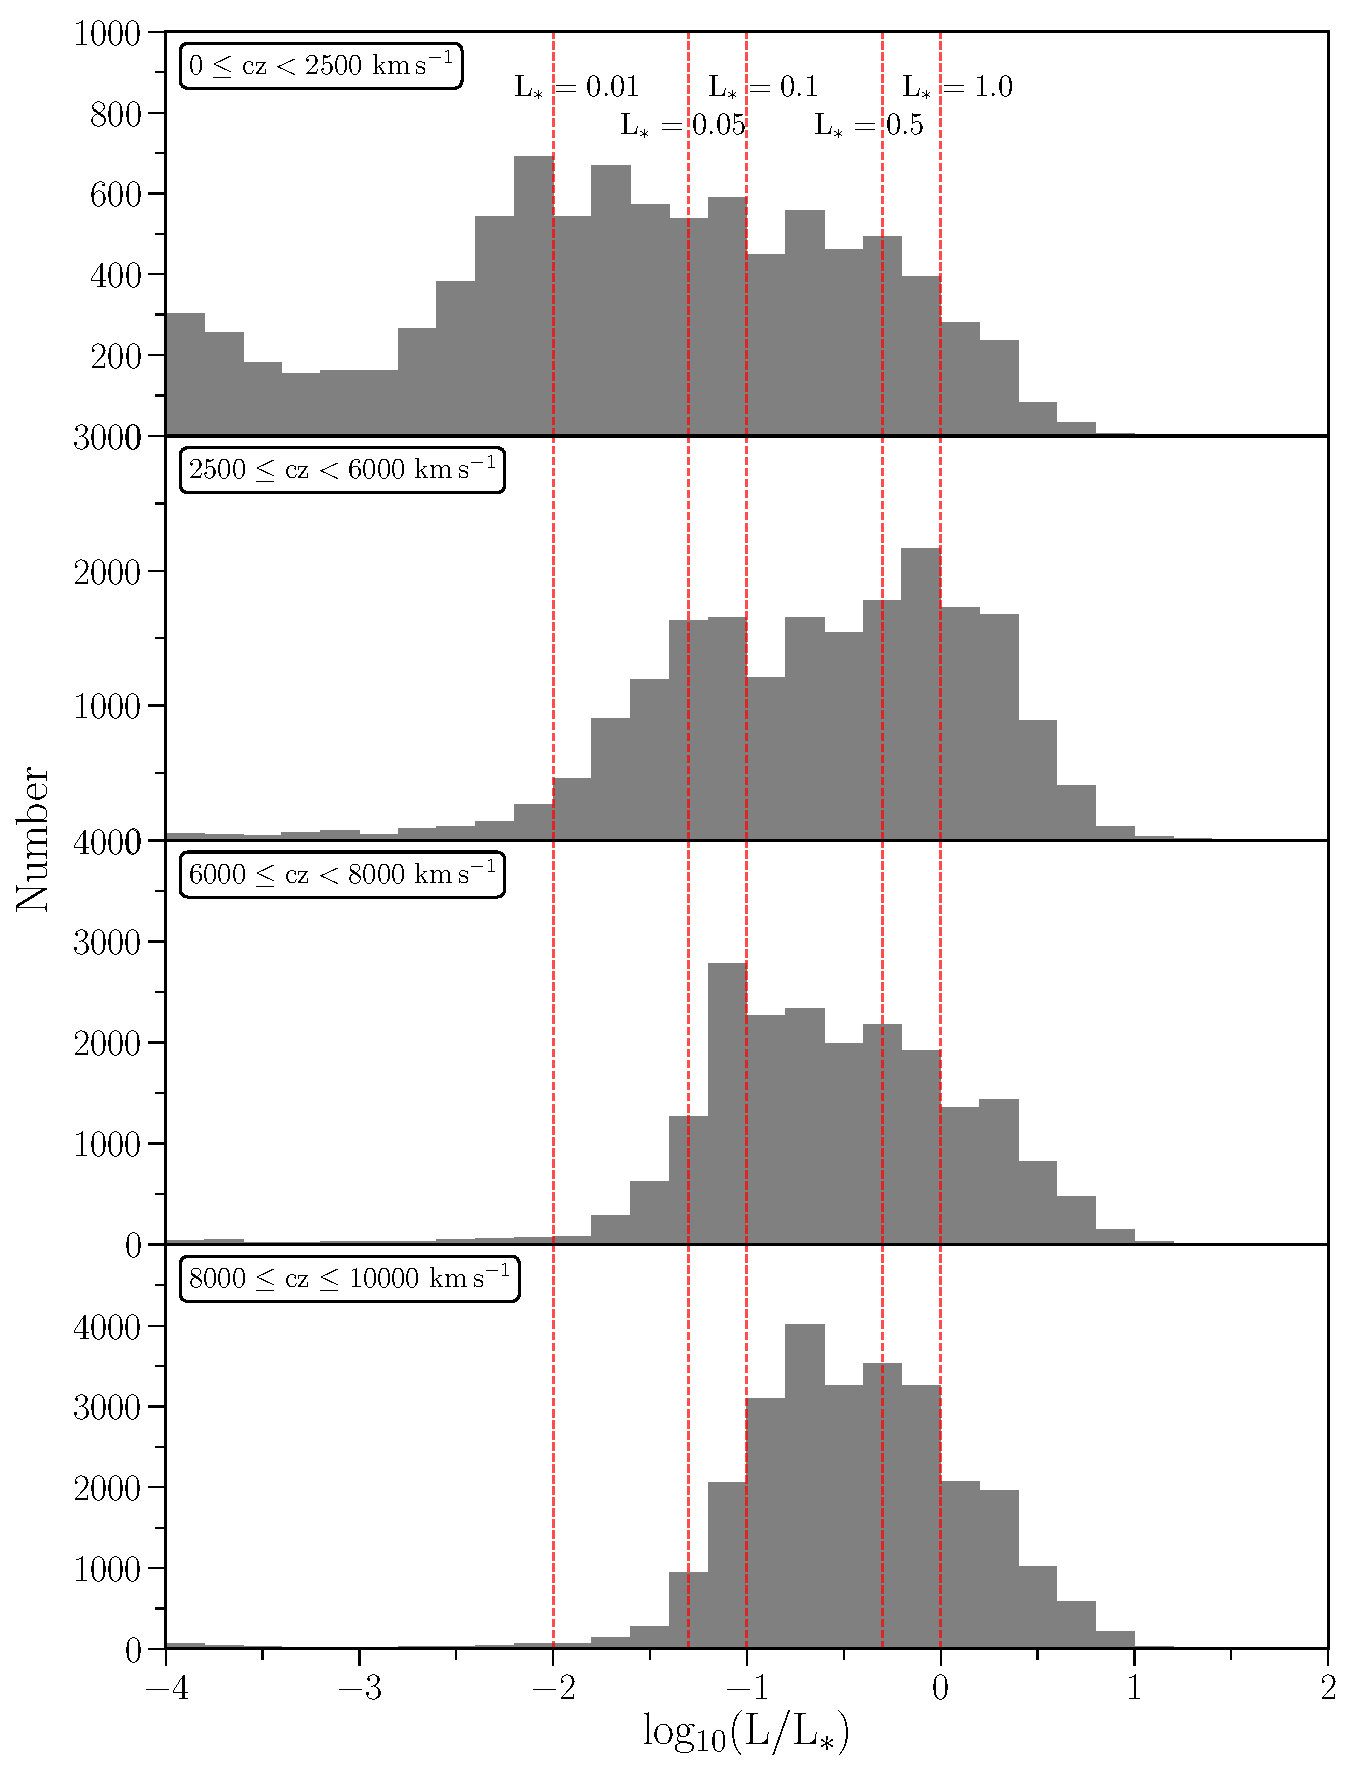
\includegraphics[width=0.50\textwidth]{fig1.pdf}
        \caption{\small{Distribution of $L/L_{\**}$ values for all galaxies in the dataset. Black vertical lines highlight 1, 0.5, 0.1, 0.05 and 0.01 $L_{\**}$. The turnoff around 0.1$L_{\**}$ shows that on average, the dataset is complete to 0.1$L_{\**}$.}}
%        \vspace{-5pt}
        \label{completeness}
\end{figure} 

The galaxy dataset contains over 108,000 entries, and includes data from SDSS, 2MASS, 2dF, 6dF, RC3, and many other, smaller surveys. Our criteria for including a galaxy in this dataset is only an accurate, spectroscopic redshift which places the galaxy in the $cz \leq 10,000$ \kms velocity range. This restriction leads to a completeness limit of $B \lesssim 18.7$ mag, or $\sim0.2 L_*$, at $cz = 10,000$ \kms, and progressively better towards lower velocities (see Figure \ref{completeness}). This limit will vary depending on which major surveys include a particular region of the sky. The major contributor is whether or not SDSS data is available, which begins around $cz = 5,000$ \kms. Figure \ref{completeness} is split into 4 velocity bins to illustrate this. Our data is complete down to $\sim0.1 L_*$ in the first bin, $0 \leq cz \leq 2,500$ \kms. At slightly higher velocity, $2500 \leq cz \leq 6000$ \kms, the completeness falls to barely better than $\sim1.0 L_*$ as we move past the near and well studied galaxies, but have yet to reach the footprint of deep all sky surveys. SDSS data becomes available in the last two bins, spanning $6000 \leq cz \leq 10,000$ \kms, and correspondingly completeness remains high down to the SDSS limits of $B \lesssim 18.7$ mag, or $\sim0.2 L_*$ at $cz = 10,000$ \kms.


\subsection{Distances \& Velocities}
For \textbf{XXXX}\% of galaxies, a redshift-independent distance estimate is available. In this case $d_{best}$ is set to the mean of all available redshift-independent distance estimates, and $derr_{best}$ is set to the standard deviation on the mean. When only a redshift is available, we set $d_{best}$ equal to the Hubble law distance as calculated with $H_0 = 71$ \kms $~\rm Mpc^{-1}$, and $derr_{best}$ equal to 10\% of the resulting distance estimate. Nearby, the uncertainty is dominated by deviations from the Hubble Flow due to, e.g., the Local Group, and at larger distances the uncertainty in $H_0$ becomes dominant. The distance error for any particular galaxy is difficult to ascertain, but at 10\% error should contain the true $1-\sigma$ error across our full redshift range.

All galaxies with zero or negative $v_hel$ have $d_{best}$ set to 1 Mpc, and $derr_{best}$ to 0.5 Mpc. 


\subsection{Diameters \& Position Angles}

We have homogenized the galaxy data beyond the steps taken by NED by normalizing diameter measurements to 2MASS $K$-band values. Most galaxies in NED have measures of inclination, position angle and diameter available in several different bands, so in order to make more meaningful comparisons we choose one band for all measurements. We chose 2MASS values for this because it was an all-sky survey, and represents the largest fraction of available galaxy data. Physical galaxy diameters are derived from 2MASS $K_s$ ``total" angular diameter measurements and galaxy distances. 2MASS $K_s$ ``total" diameter estimates are surface brightness extrapolation measurements and are derived as 

\begin{equation}
r_{tot} = r' + a(ln(148)^b,
\end{equation}

\noindent where $r_{tot}$ is defined as the point where the surface brightness extends to 5 disk scale lengths, $r'$ is the starting point radius ($>5" - 10"$ beyond the nucleus, or core influence), and $a$ and $b$ are Sersic exponential function scale length parameters ($f = f_0 \exp{(-r/a)}^{(1/b)}$, see Jarret et al. 2003 for a full description). Approximately $50\%$ of all the galaxies have this 2MASS $K_s$ ``total" diameter. Of the remainder, $20\%$ have SDSS diameters, $3\%$ have diameters from other surveys, and $27\%$ have no published diameter. 

For galaxies with multiple published measurements from different facilities, we have derived linear fits in order to convert between them. The orthogonal distance regression (ODR) algorithm as implemented by the Fortran code ODRPACK (and the Python wrapped version included in the Scipy package) was used to derive these best fits and their associated errors. ODR, compared to the more common linear regression algorithm, assumes errors in both x- and y-coordinates and thus minimizes the orthogonal distance between both dependent and independent data and the fit. The fits for each survey are listed in Table \ref{diameter_fits}.

A significant fraction of galaxies have irregular, incomplete, or otherwise suspect diameter data as published in NED. For example, some have 2MASS $K_s$ ``total" diameters available, but the published axis ratio significantly deviates from that found in other surveys. Furthermore, often our highest ranking diameter survey has incomplete data (such as a missing axis ratio or position angle measurement). For our purposes we want to choose a single, representative value for each parameter. We decision tree is as follows: 1) we choose the highest ranking measurement available, and choose the largest major-axis diameter value when multiple are available from the same facility, 2) we choose the highest ranking axes ratio, preferentially selecting the value from the measurement chosen in (1), but rejecting a ratio = 1 when the average ratio of all measurements is less than 1, 3) we choose the highest ranking position angle measurement, again preferentially selecting the value included in (1). The decision of diameter, ratio and position angle for each galaxy is included in the $diameter_key$ tuple.

Finally, we also compute an estimate of the virial radius of each galaxy as $log R_{vir} = 0.69 log D + 1.24$. This follows the parametrization of Stocke et al. (2013) relating a galaxy's luminosity to its virial radius, and the Wakker $\&$ Savage (2009) empirical relation between diameter and luminosity (see Wakker et al. 2015 and references therein for further details). Errors are propagated from the original published magnitude errors.


\begin{table}[ht]\footnotesize
\begin{center}
\begin{tabular}{l c c c}
 \hline \hline
 Survey Name                			& m   				& y-intercept			& Fraction of Total	\\
  \hline \hline 
K\_s (2MASS isophotal)			& $1.765 \pm 0.003$		& $1.31 \pm 0.06$		&	XXX			\\
POSS1 103a-O					& $0.869 \pm  0.007$	& $17.6 \pm 0.4$						\\
POSS1 103a-E					& $1.055 \pm 0.043$		& $26.22 \pm 1.98$		&	XXX			\\
ESO-LV "Quick Blue" IIa-O		& $0.81 \pm 0.02$		& $-9.7 \pm 1.4$		&	XXX			\\
r (SDSS Isophotal)				& $1.033 \pm 0.005$		& $0.84 \pm 0.17$		&	XXX			\\
RC3 D\_0 (blue)				& $1.040 \pm 0.009$		& $1.29 \pm 0.58$		&	XXX			\\
RC3 D\_25, R\_25 (blue)			& $1.107 \pm 0.009$		& $3.09 \pm 0.60$		&	XXX			\\
r (SDSS Petrosian)				& $4.728 \pm 0.032$		& $3.38 \pm 0.21$		&	XXX			\\
r (SDSS deVaucouleurs)			& $3.49 \pm 0.04$		& $14.45 \pm 0.21$		&	XXX			\\
r (SDSS de Vaucouleurs)			& $2.70 \pm 0.04$		& $15.64 \pm 0.22$		&	XXX			\\
RC3 A\_e (Johnson B)			& $2.25 \pm 0.06$		& $19.2 \pm 1.8$		&	XXX			\\
r (SDSS Exponential)			& $8.24 \pm 0.06$		& $7.7 \pm 0.2$		&	XXX			\\
B (Johnson)					& $1.24 \pm 0.09$		& $-25.3 \pm 9.7$		&	XXX			\\
R (Kron-Cousins)				& $1.47 \pm 0.14$		& $-35.9 \pm 14.4$		&	XXX			\\
ESO-Uppsala "Quick Blue" IIa-O	& $1.06 \pm 0.02$		& $-13.4 \pm 1.4$		&	XXX			\\
ESO-LV IIIa-F					& $4.65 \pm 0.13$		& $23.02 \pm 0.92$		&	XXX			\\
\hline
\end{tabular}
\end{center}
  \caption{\small{Diameter fits in order of quality.}}
  \label{diameter_fits}
\end{table}


\subsection{Photometry}
For each galaxy we retrieved all B-band and SDSS $g$, $r$, and $z$ measurements. Direct $B$ band measurements are available for $\sim 30\%$ of galaxies, and most of the rest have SDSS magnitudes, which we converted to $B$-band via $B = g + 0.39 (g-r) + 0.21$ (Jester et al. 2005). Per SDSS DR12 guidelines, we preferentially selected SDSS $petrosian$ magnitudes when available, followed by $model$ and $cmodel$ values if $petrosian$ was not available. We then selected the min, max and median $B$-band values when more than one was available for inclusion in the final data product. SDSS-converted $B$-band values are included as a separate estimate. 

We then computed each galaxy's luminosity in units of $L_{\**}$ for each of the min, median, max and SDSS $B$-band values as follows:

\begin{equation}
	\frac{L}{L_{\**}} = 10^{-0.4 (M_{B} - M_{B_{\**}})},
	\label{lstar}
\end{equation}

where $M_B$ is the galaxy absolute magnitude, calculated using the $d_{best}$ distance estimate as described above. We adopted the CfA galaxy luminosity function by Marzke et al. (1994), which sets $B_{\**} $ = -19.57. 


%\begin{figure}[ht!]
%        \centering
%        \includegraphics[width=0.48\textwidth]{hist(azimuth)_overlaid_all.pdf}
%        \caption{\small{The distributions of azimuth angles for red and blue-shifted samples, with the combined sample plotted in black. $Azimuth = 0$ corresponds to along the projected major axis of the galaxy, and $azimuth = 90$ is along the minor axis.}}
%        \label{azimuth_dist}
%        \vspace{5pt}
%\end{figure} 


\section{The Catalog}
The galaxy catalog columns contain the following information.

\begin{enumerate}

\item \textit{preferredName} - Our preferred name for the galaxy. The ordering is as follows: MESSIER, NGC, MRK, UGC, PHL, 3C, IC, SBS, MCG, ISO, TON, PGC, PG, PB, FGC, HS, HE, KUG, IRAS, RX, CGCG, FBQS, LBQS, SDSS, VCC, 2MASS, 2DF, 6DF, HIPASS, 2MASX. If none of these are available, the first NED name is adopted.

\item \textit{NEDname} - The preferred name for the galaxy in the NED database.

\item \textit{z} - NED redshift for the galaxy. 

\item \textit{degreesJ200RA\_Dec} - Equatorial coordinates in degrees (J2000.0 epoch).

\item \textit{J2000RA\_Dec} - Equatorial coordinates in (HH, MM, SS), (DD, MM, SS) format (J2000.0 epoch).

\item \textit{galacticLong\_Lat} - Galactic longitude and latitude coordinates.

\item \textit{helioVelocity} - Heliocentric radial velocity in \kms units.

\item \textit{vcorr} - Virgocentric flow-corrected velocity. Following Geller \& Huchra (1982), this corresponds to a 300 \kms velocity toward $R.A. = 186^{\circ}.7833$, $decl. = 12^{\circ}.9333$.

\item \textit{distvcorr} - Distance calculated from $vcorr$ with a Hubble constant of $H_0 = 71$ \kms $~\rm Mpc^{-1}$.

\item \textit{RID\_mean} - Mean redshift independent distance from the NED-D catalog.

\item \textit{RID\_std} - Standard deviation of all redshift independent distance measurements.

\item \textit{RID\_min} - Minimum published redshift independent distance.

\item \textit{RID\_max} - Maximum published redshift independent distance.

\item \textit{$dist\_best$} - Our chosen best distance estimate. $dist\_best$ is equal to $RID_mean$ when a redshift independent distance is available, and otherwise defaults to $distvcorr$.

\item \textit{distErr} - The error on $best\_dist$. $distErr$ is equal to $RID_std$ when a redshift independent distance is available. Otherwise, $distErr$ is set to 10\% of $distvcorr$ when $vcorr \geq 0$, and 50\% of $distvcorr$ if $vcorr < 0$.

\item \textit{angD} - Major and minor axis diameters in units of arcsec. 

\item \textit{$angD\_err$} - Angular diameter errors. 

\item \textit{linD} - Linear major and minor axis diameters in units of kpc, calculated using $best\_dist$.

\item \textit{linD\_err} - Linear diameter errors.

\item \textit{inc} - Galaxy inclination calculated as $inc. = \cos^{-1} (minor / major)$ in units of degrees.

\item \textit{adjustedInc} - Galaxy inclination calculated assuming a finite disk thickness following Heidmann et al. (1972a):

\begin{equation}
	\cos(i) = \sqrt{\frac{q^2 - q_0^2}{1 - q_0^2}},
	\label{incEq}
\end{equation}

\item \textit{incErr} - Inclination error derived from the reported error in the ratio between angular major and minor axes.

\item \textit{PA} - Position angle in units of degrees.

\item \textit{diam\_key} - The observed passband of the diameter measurements. The published diameters are converted to an equivalent 2MASS $K_s$ ``total" value following the fits given in \ref{diameter_fits}.

\item \textit{ratio\_key} - The observed passband of the diameter ratio measurement. This is used to calculate the minor axis diameters and inclinations.

\item \textit{pa\_key} - The observed passband of the position angle measurement. 

\item \textit{RC3\_type} - Galaxy morphology as published in the Third Reference Catalog of Bright Galaxies (RC3; see de Vaucouleurs G. et al. 1994 for full description). Galaxies not included in RC3 are marked '-99'.

\item \textit{RC3\_d25} - The RC3 apparent major isophotal diameter measured at the 25th magnitude surface-brightness level, in units of B-mag per arcsecond.

\item \textit{RC3\_r25} - The RC3 ratio of the major to minor axis diameter (converted from decimal logarithm to a straight ratio in order to match the units of $ratio\_key$). 

\item \textit{RC3\_pa} - The RC3 position angle in units of degrees.

\item \textit{groups} - 

\item \textit{morphology} - 

\item \textit{distIndicator} - 

\item \textit{luminosityClass} - 

\item \textit{E(B-V)} - Galactic mean dust extinction in the direction of each galaxy from Schlafly and Finkbeiner (2011).

\item \textit{B\_mag} - 

\item \textit{B\_median} - The median B-band magnitude.

\item \textit{B\_max} - The brightest B-band magnitude available in NED for this object.

\item \textit{B\_min} - The dimmest B-band magnitude available in NED for this object.

\item \textit{B\_sdss} - SDSS $g$ and $r$-band measurements converted to $B$-band via $B = g + 0.39 (g-r) + 0.21$ (Jester et al. 2005).

\item \textit{g\_sdss} - The SDSS $g$-band magnitude used in the $B\_sdss$ calculation.

\item \textit{r\_sdss} -The SDSS $r$-band magnitude used in the $B\_sdss$ calculation.

\item \textit{z\_sdss} - SDSS $z$-band magnitude.

\item \textit{Lstar\_median} - The $L / L_{\**}$ ratio calculated using $B\_median$, $dist\_best$, and $E(B-V)$ following Eq. \ref{lstar}.

\item \textit{Lstar\_max} - The $L / L_{\**}$ ratio calculated using $B\_max$, $dist\_best$ + $dist\_err$, and $E(B-V)$ following Eq. \ref{lstar}.

\item \textit{Lstar\_min} - The $L / L_{\**}$ ratio calculated using $B\_min$, $dist\_best$ - $dist\_err$, and $E(B-V)$ following Eq. \ref{lstar}.

\item \textit{altNames} - The NED list of alternative object names for this galaxy with spaces removed.


\end{enumerate}


\section{Summary}

Summary...


This research has made use of the NASA/IPAC Extragalactic Database (NED) which is operated by the Jet Propulsion Laboratory, California Institute of Technology, under contract with the National Aeronautics and Space Administration. Based on observations with the NASA/ESA \textit{Hubble Space Telescope}, obtained at the Space Telescope Institute, which is operated by AURA, Inc., under NASA contract NAS 5-26555.


\nocite{*}
\bibliography{paper_bib}
\bibliographystyle{apj}

\end{document}
